
\chapter{Arquitecturas y Enfoques Actuales en Text-to-Query}
\label{chap:stateoftheart}

El capítulo anterior presentó los fundamentos necesarios para comprender la generación \emph{text-to-query}: los modelos de lenguaje, las limitaciones de estos, las representaciones intermedias, los mecanismos de verificación y el estándar híbrido \ac{SQL}/\ac{PGQ}. A partir de esa base, este capítulo revisa los trabajos actuales en sistemas \emph{text-to-query}.

Esta revisión no se plantea como una lista cronológica de trabajos, sino como un análisis organizado por dimensiones, decisión tomada dado que la literatura reciente aborda el problema desde criterios diversos: algunas revisiones clasifican los sistemas según la arquitectura del modelo, otras según las etapa del \emph{pipeline}, e incluso según la estrategia de \emph{prompting} empleada~\cite{NLinterfaces}, entre otros. Aunque estas clasificaciones son útiles, no siempre permiten comparar los trabajos bajo criterios comunes ni identificar con claridad las brechas de investigación.

Por ello, este capítulo adopta una taxonomía multidimensional para analizar la literatura de manera más ordenada.

\section{Marco taxonómico del análisis}
\label{sec:sota-taxonomia}

Resolver el problema \emph{text-to-query} obliga a considerar simultáneamente decisiones de: aprendizaje, orquestación arquitectónica, representación, enriquecimiento contextual y criterios de verificación. Estas decisiones operan en diferentes niveles y etapas, incluyendo combinaciones muy variadas en la literatura \cite{hong2024llmtext2sql,shi2025surveyllmtext2sql,liu2025nli4db}. 

En base a esta complejidad y vacío identificado, se desarrolló una taxonomía con seis dimensiones complementarias para clasificar los sistemas \emph{text-to-query}. La taxonomía presentada fue elaborada recogiendo y reorganizando ejes ya presentes en surveys recientes \cite{hong2024llmtext2sql,liu2024nl2sqlsurvey,shi2025surveyllmtext2sql,qin2022recentadvances},
y añadiendo dos contribuciones específicas, producto de la revisión de literatura y de los patrones observados: separar el \emph{paradigma de razonamiento} y las \emph{propiedades de evaluación} como dimensiones independientes, de forma tal que un mismo trabajo pueda recibir etiquetas en cada eje sin que las etiquetas de uno predetermine las del otro.

\begin{figure}[h]
    \centering
    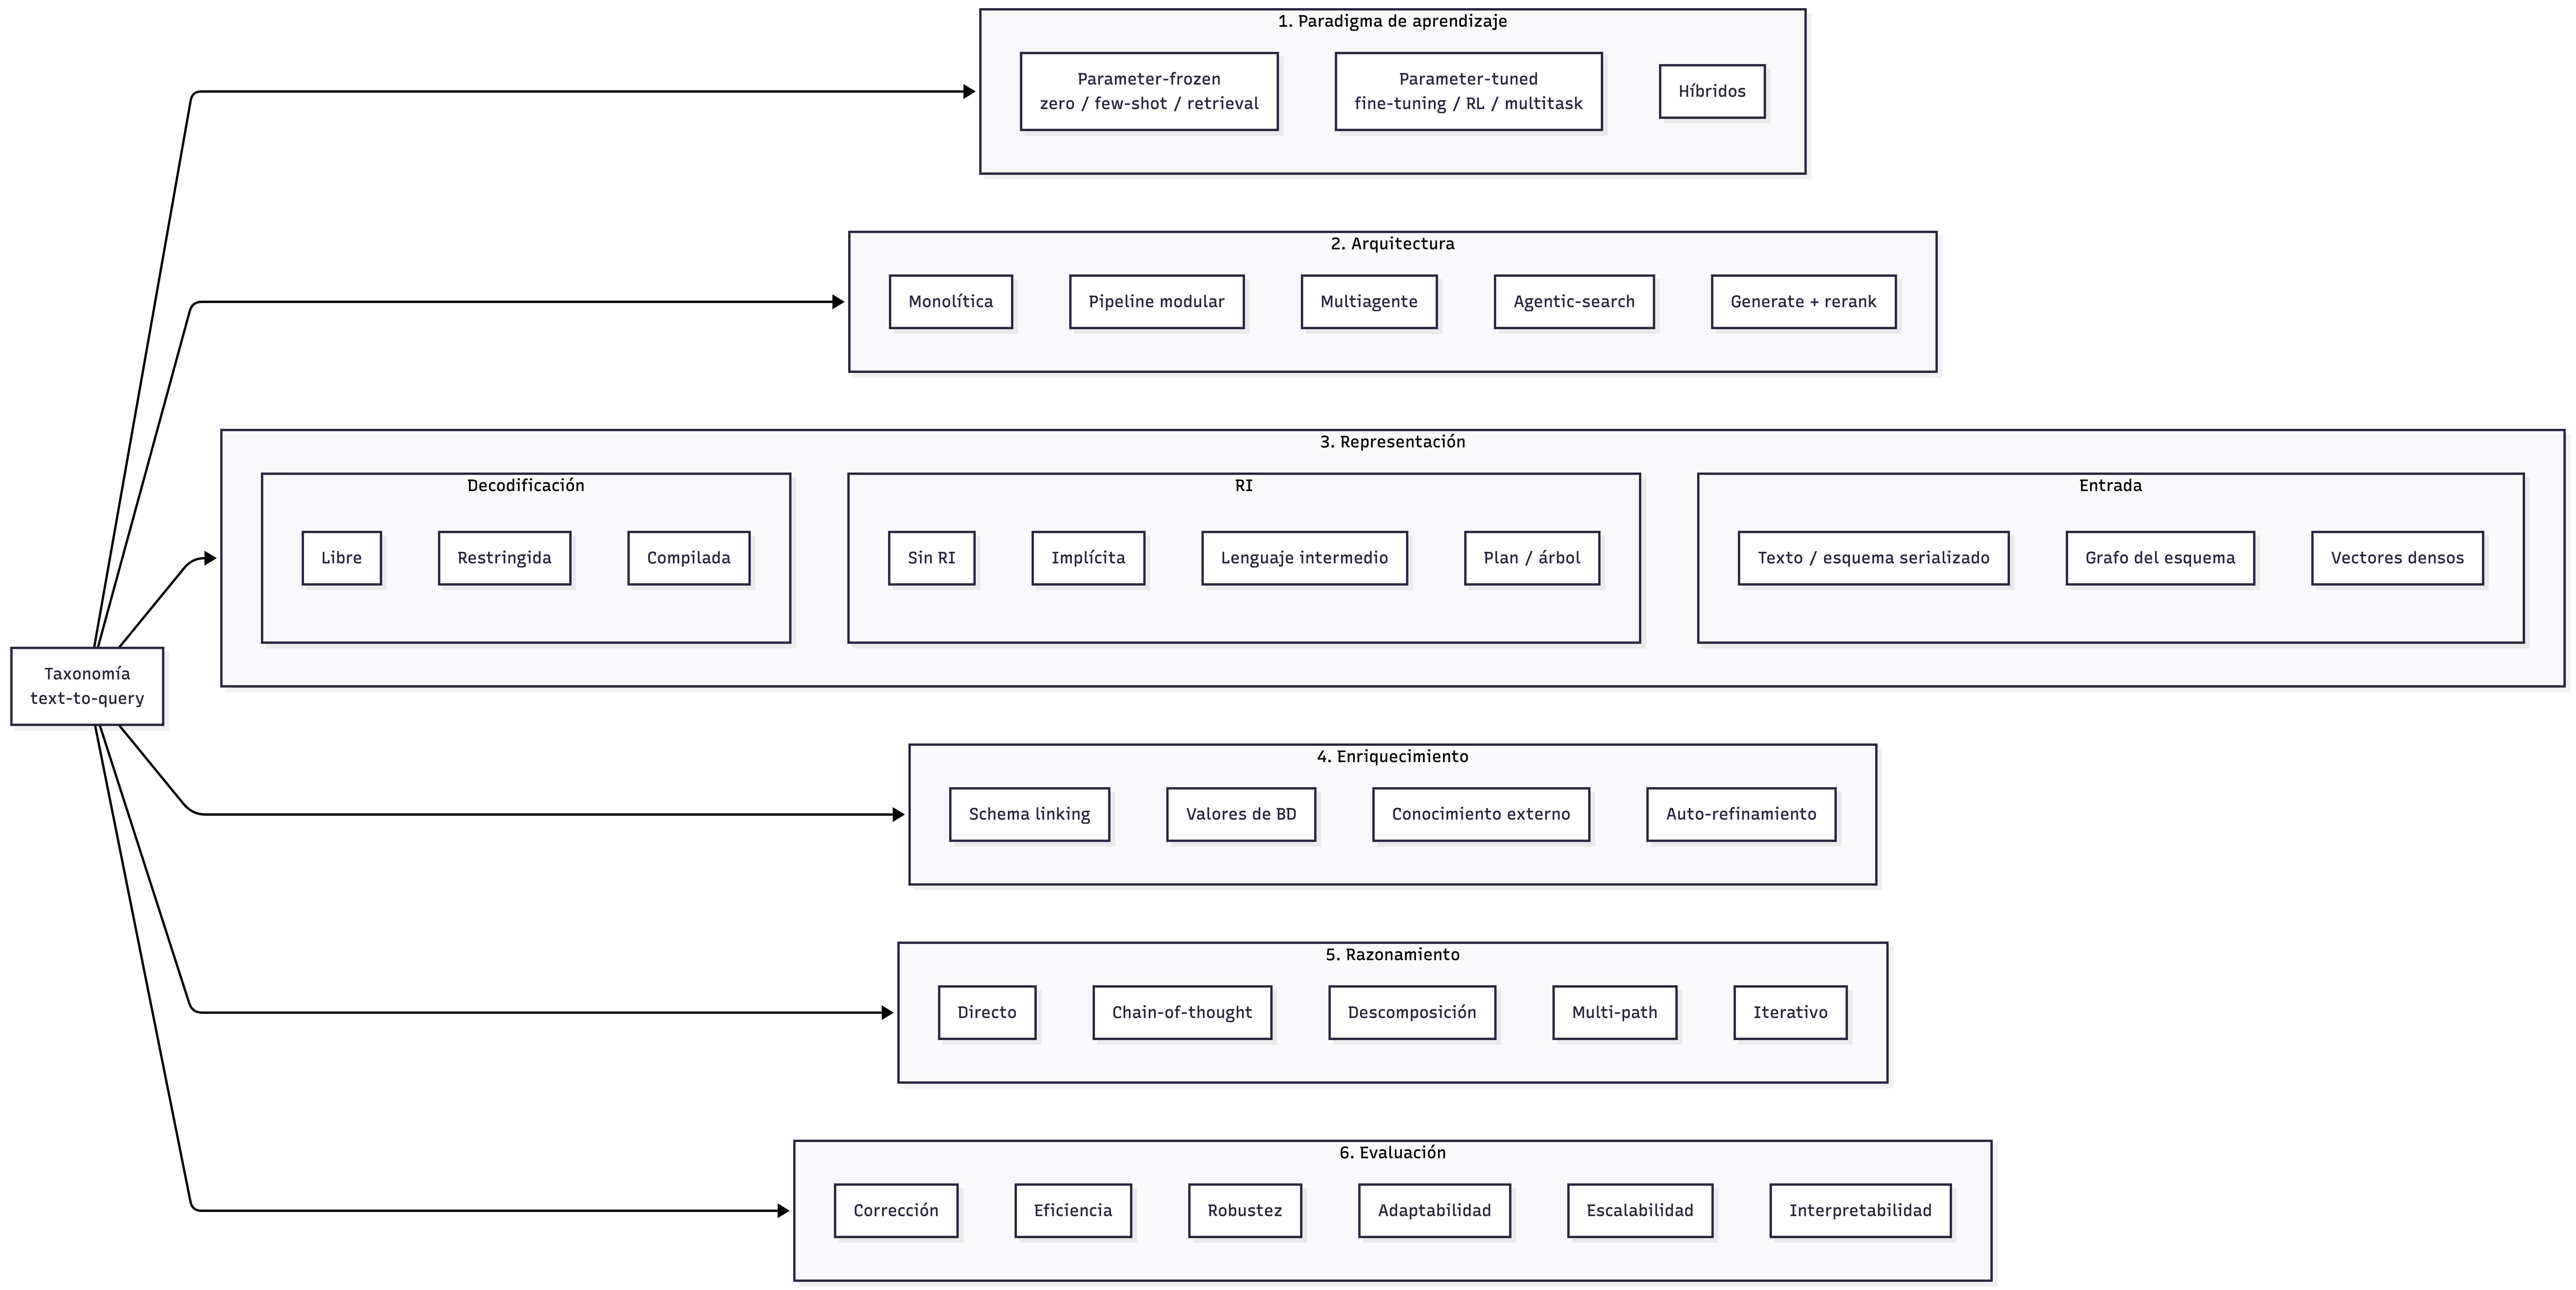
\includegraphics[width=\linewidth]{figs/Chap3/Taxonomía.png}
    \caption{Taxonomía multidimensional propuesta. Cada uno de los seis ejes
    ortogonales agrupa las decisiones de diseño observadas en la literatura
    de \emph{text-to-query} y sus principales subcategorías.}
    \label{fig:taxonomia}
\end{figure}

La Figura~\ref{fig:taxonomia} sintetiza las seis dimensiones consideradas,
cuya descripción y justificación se resumen a continuación:

\begin{enumerate}
    \item \textbf{Paradigma de aprendizaje:} Abarca cómo se adapta el modelo base a la tarea, ya sea con parámetros congelados (\emph{zero-shot}, \emph{few-shot} estático o con recuperación dinámica), parámetros ajustados (\emph{fine-tuning}, preentrenamiento continuo, aprendizaje multi-tarea o por refuerzo) o estrategias híbridas. Esta dimensión ayuda a determinar el costo de adaptación, la dependencia de datos anotados y la complejidad de transferencia a nuevos dominios.

    \item \textbf{Arquitectura del sistema:} La distribución de la ejecución entre el modelo y los diferentes módulos auxiliares, distinguiendo configuraciones monolíticas, \emph{pipelines} modulares, multiagente, \emph{agentic-search} y generación con reordenamiento.

    \item \textbf{Representación:} Las estructuras que median entre la pregunta y la consulta final, considerando codificación de la entrada, representación intermedia y estrategia de decodificación.

    \item \textbf{Mecanismos de enriquecimiento contextual:} La información adicional que ancla la salida al esquema y al dominio, incluyendo \emph{schema linking}, recuperación de contenido de la base de datos, conocimiento externo o ciclos de auto-refinamiento. Se trata como dimensión propia porque su efecto sobre la corrección actúa de forma transversal a la arquitectura y al paradigma de aprendizaje.

    \item \textbf{Paradigma de razonamiento:} Cómo se estructura la inferencia que lleva a la consulta, en variantes directa, en cadena de pensamiento, descompositiva, de múltiples caminos o de retroalimentación iterativa.

    \item \textbf{Evaluación:} Las propiedades del sistema que prioriza explícitamente cada trabajo, entre corrección, eficiencia, robustez, adaptabilidad, escalabilidad e interpretabilidad. Se incorpora como eje independiente para hacer visible el sesgo dominante hacia la corrección y permitir comparaciones sobre propiedades críticas en consultas empresariales.
\end{enumerate}

A partir de esta categorización, las siguientes secciones revisarán la literatura reciente analizando, por dimensión, cómo se han posicionado los trabajos más representativos, enfocándose en propuestas publicadas mayoritariamente entre 2017 y 2026, abarcando de esta forma, desde los primeros sistemas neuronales basados en codificadores especializados hasta las arquitecturas multiagente más recientes.

\section{Paradigma de aprendizaje}
\label{sec:sota-d1-aprendizaje}

Esta sección analiza la forma en que los sistemas \emph{text-to-query} adaptan su modelo base a la tarea, ya que si bien la mayoría de los trabajos revisados utiliza \acp{LLM} o modelos preentrenados de tipo \emph{encoder-decoder}, no todos los sistemas los emplean de la misma manera.









En términos generales, pueden distinguirse tres estrategias principales: La primera consiste en mantener los parámetros del modelo congelados y adaptar su comportamiento únicamente mediante el \emph{prompt}. La segunda ajusta los parámetros del modelo mediante \emph{fine-tuning} u otros procesos de entrenamiento adicional. La tercera combina ambas aproximaciones, por ejemplo, usando modelos congelados para ciertas etapas del \emph{pipeline} y componentes ajustados para tareas específicas como selección, reordenamiento o verificación.

Esta distinción es relevante porque cada estrategia implica compromisos distintos en términos de costo de adaptación, necesidad de datos anotados, flexibilidad frente a nuevos dominios y control sobre el comportamiento del sistema.

\subsection{Aprendizaje con parámetros congelados}
\label{subsec:sota-d1-frozen}

En esta categoría, la adaptación a la tarea se realiza únicamente mediante el diseño del \emph{prompt}, sin modificar los parámetros internos del modelo. Por tanto, la diferencia principal entre los enfoques no está en el entrenamiento del modelo, sino en la forma en que se construye el contexto que se entrega para generar la consulta.

\paragraph{(a) \emph{Zero-shot}.} 
Los enfoques \emph{zero-shot} prescinden de ejemplos demostrativos y se apoyan solo en la pregunta del usuario, la descripción del esquema y las instrucciones incluidas en el \emph{prompt}. C3-SQL~\cite{C3-SQL2023} es representativo de esta línea, ya que muestra que un \emph{prompt} cuidadosamente diseñado puede alcanzar resultados competitivos sobre Spider sin incorporar ejemplos previos. De manera similar, Alpha-SQL~\cite{Alpha-SQL2025}, aunque corresponde a una arquitectura agéntica, puede considerarse \emph{zero-shot} porque no depende de demostraciones específicas del dominio; en su lugar, explora el espacio de consultas mediante búsqueda guiada sobre \emph{prompts} dinámicos.

La principal ventaja de esta subcategoría es su bajo costo de adaptación, pues no requiere datos anotados ni selección de ejemplos. Sin embargo, su desempeño depende fuertemente de la capacidad del modelo base y tiende a degradarse cuando el esquema es grande, poco convencional o presenta relaciones difíciles de inferir solo a partir de su descripción.

\paragraph{(b) \emph{Few-shot in-context learning}.} 
La mayoría de los sistemas recientes basados en \acp{LLM} se ubica en esta subcategoría. En estos enfoques, el modelo recibe un conjunto de ejemplos de pares pregunta-consulta que ilustran el comportamiento esperado. Estos ejemplos pueden ayudar al modelo a reconocer patrones de formulación, estructuras frecuentes de consulta y formas adecuadas de vincular la pregunta con el esquema.

DIN-SQL~\cite{DIN-SQL2023} es uno de los trabajos influyentes en esta línea. Su propuesta descompone la tarea en subpasos y diseña \emph{prompts} específicos para cada uno, apoyados en ejemplos seleccionados manualmente. Enfoques posteriores o relacionados, como DAIL-SQL~\cite{DAIL-SQL2023}, ACT-SQL~\cite{ACT-SQL2023}, PET-SQL~\cite{PET-SQL2024}, DEA-SQL~\cite{DEA-SQL2024}, RSL-SQL~\cite{RSL-SQL2024}, CHESS~\cite{CHESS2024}, MAC-SQL~\cite{MAC-SQL2023}, TA-SQL~\cite{TA-SQL2024}, CoE-SQL~\cite{CoE-SQL2024}, PURPLE~\cite{PURPLE2024}, ODIS~\cite{ODIS2023}, Gen-SQL~\cite{Gen-SQL2025}, SGU-SQL~\cite{SGU-SQL2025}, CRED-SQL~\cite{CRED-SQL2025} y CRUSH4SQL~\cite{CRUSH4SQL2023}, entre otros, mantienen esta lógica general, aunque la combinan con distintas formas de descomposición, recuperación, verificación o refinamiento.

La amplitud de trabajos en esta subcategoría muestra la madurez del paradigma de aprendizaje en contexto. No obstante, también evidencia una limitación: muchas mejoras dependen de ajustes en la ingeniería de \emph{prompts}, la selección de ejemplos o la organización del contexto, más que de cambios profundos en la arquitectura del sistema.

\paragraph{(c) Aprendizaje en contexto dinámico con recuperación.} 
Una variante más flexible del \emph{few-shot} consiste en seleccionar dinámicamente los ejemplos que se incluyen en el \emph{prompt}. En lugar de usar un conjunto fijo de demostraciones, el sistema recupera ejemplos similares a la pregunta de entrada o al esquema objetivo. Esta estrategia busca que el contexto proporcionado al modelo sea más relevante para cada caso particular.

OpenSearch-SQL~\cite{OpenSearch-SQL2025} ilustra esta aproximación mediante un módulo dedicado a la recuperación de ejemplos. CRED-SQL~\cite{CRED-SQL2025} también contempla esta estrategia como una extensión posible dentro de su arquitectura. La ventaja principal frente al \emph{few-shot} estático es su mayor adaptabilidad a dominios heterogéneos. Sin embargo, esta adaptabilidad depende de la calidad, cobertura y organización del corpus de ejemplos disponible. Si los ejemplos recuperados son poco representativos o introducen patrones incorrectos, el desempeño del modelo puede verse afectado.

\subsection{Aprendizaje con parámetros ajustados}
\label{subsec:sota-d1-tuned}

En esta categoría se modifican los parámetros del modelo mediante
entrenamiento adicional sobre datos específicos de la tarea. Es la familia
históricamente más extendida en \emph{text-to-SQL} previa al auge de los
\acp{LLM} de propósito general.

\paragraph{(a) Fine-tuning supervisado.} Trabajos como
Seq2SQL~\cite{Seq2SQL2017}, BRIDGE~\cite{BRIDGE2020},
RAT-SQL~\cite{RAT-SQL2021}, SmBoP~\cite{SmBoP2021},
RaSaP~\cite{RaSaP2021}, SHiP~\cite{SHiP2022},
RASAT~\cite{RASAT2022}, PICARD~\cite{PICARD2022},
S²SQL~\cite{S2SQL2022}, Graphix-T5~\cite{Graphix-T52022},
RESDSQL~\cite{RESDSQL2023}, T5-3B+NatSQL~\cite{T5-3B+NatSQL+TokenPreprocessing2023},
SQLFormer~\cite{SQLFormer2023}, CatSQL~\cite{CatSQL2023} y
DTS-SQL~\cite{DTS-SQL2024} ajustan modelos completos sobre conjuntos como
Spider o WikiSQL. Las arquitecturas base varían desde redes específicas para
\emph{text-to-SQL} (Seq2SQL, BRIDGE, RAT-SQL, SmBoP) hasta variantes de T5
adaptadas (PICARD, RESDSQL, Graphix-T5). Los sistemas de esta sub-categoría
dominaron los rankings de los benchmarks controlados durante el período
pre-LLM (2017--2022); su costo de entrenamiento y su dependencia del dominio
de entrenamiento limitan, sin embargo, su transferencia directa a entornos
empresariales.

\paragraph{(b) Preentrenamiento continuo.} CodeS~\cite{CodeS2024} representa
una variante intermedia: parte de un modelo de código preentrenado de
propósito general y aplica preentrenamiento continuo sobre un corpus
masivo orientado a SQL antes del \emph{fine-tuning} supervisado final. La
estrategia mejora la transferencia a dominios desconocidos, pero requiere
infraestructura considerable y un corpus de entrenamiento curado.

\paragraph{(c) Aprendizaje multi-tarea.} Algunos trabajos entrenan el modelo
sobre varias tareas relacionadas para mejorar la generalización.
TKK~\cite{TKK2022} aborda \emph{text-to-SQL} junto con tareas auxiliares
de comprensión de esquema. ROUTE~\cite{ROUTE2025} adopta el aprendizaje
multi-tarea como principio organizador del \emph{fine-tuning},
integrando tareas de generación, corrección y razonamiento sobre esquemas.
PARSQL~\cite{PARSQL2025} sigue una línea similar al combinar generación con
selección entre candidatos. La motivación común es que las tareas auxiliares
fuerzan al modelo a desarrollar representaciones internas más robustas del
esquema y de la sintaxis SQL.

\paragraph{(d) Aprendizaje por refuerzo.} STRuCT-LLM~\cite{STRuCT-LLM2025}
incorpora aprendizaje por refuerzo para alinear la generación con
señales de ejecución y con tareas de razonamiento sobre tablas y grafos
simultáneamente. Seq2SQL~\cite{Seq2SQL2017}, en una época mucho más
temprana, ya empleaba aprendizaje por refuerzo basado en la recompensa de
ejecución. La adopción del paradigma sigue siendo minoritaria pero ha
resurgido con fuerza en propuestas recientes orientadas a unificar
razonamiento estructurado con generación.

\subsection{Estrategias híbridas}
\label{subsec:sota-d1-hibridas}

Una fracción creciente de los sistemas más recientes combina componentes
con parámetros congelados y componentes ajustados.
XiYan-SQL~\cite{XiYan-SQL2024} adopta una arquitectura multiagente en la que
un generador puede ser un \ac{LLM} ajustado de la familia
XiYanSQL-QwenCoder mientras que módulos auxiliares operan
\emph{in-context}. CHASE-SQL~\cite{CHASE-SQL2025} combina generadores
\emph{in-context} con un seleccionador entrenado mediante \emph{fine-tuning}.
ZeroNL2SQL~\cite{ZeroNL2SQL2024} distribuye la carga entre un modelo
preentrenado pequeño y un \ac{LLM} congelado. MetaSQL~\cite{MetaSQL2024}
aplica un esquema análogo en la fase de selección sobre múltiples
candidatos. La motivación es pragmática: aprovechar la capacidad de
generalización de los \acp{LLM} sin renunciar al control fino que provee
el ajuste sobre los componentes críticos.

\subsection{Observaciones críticas}
\label{subsec:sota-d1-obs}

La revisión de esta dimensión muestra un desplazamiento progresivo del
\emph{fine-tuning} de extremo a extremo hacia configuraciones híbridas
y \emph{in-context}. Esta tendencia es coherente con el aumento del costo
computacional asociado al entrenamiento de \acp{LLM} de gran tamaño. Sin
embargo, los sistemas puramente \emph{in-context} acumulan dos
limitaciones recurrentes: dependencia fuerte del modelo subyacente, lo
que dificulta auditar el sistema desde el punto de vista de gobernanza, y
ausencia de mecanismos formales para garantizar que la salida respete
el esquema. La investigación de la presente tesis se posiciona como
agnóstica al paradigma de aprendizaje subyacente: el énfasis se traslada
a la representación intermedia y al bucle de verificación, de modo que
la corrección estructural no descanse exclusivamente en la calidad
estadística del generador.

\section{Arquitectura del Sistema}
\label{sec:sota-d2-arquitectura}

Esta sección describe cómo se organiza el cómputo en los sistemas
\emph{text-to-query}. La distinción es independiente del paradigma de
aprendizaje: un mismo paradigma puede dar lugar a arquitecturas
monolíticas, modulares, multiagente, agénticas o de generación con
reordenamiento.

\subsection{Arquitecturas monolíticas}
\label{subsec:sota-d2-monoliticas}

En las arquitecturas monolíticas, una sola invocación del modelo produce
la consulta completa. Es la configuración natural de los sistemas
\emph{end-to-end} entrenados para mapear pregunta a consulta directamente.
Pertenecen a esta categoría Seq2SQL~\cite{Seq2SQL2017},
BRIDGE~\cite{BRIDGE2020}, RAT-SQL~\cite{RAT-SQL2021},
SmBoP~\cite{SmBoP2021}, RaSaP~\cite{RaSaP2021}, RASAT~\cite{RASAT2022},
PICARD~\cite{PICARD2022}, S²SQL~\cite{S2SQL2022},
Graphix-T5~\cite{Graphix-T52022}, T5-3B+NatSQL~\cite{T5-3B+NatSQL+TokenPreprocessing2023},
SQLFormer~\cite{SQLFormer2023}, CatSQL~\cite{CatSQL2023},
SHiP~\cite{SHiP2022}, CodeS~\cite{CodeS2024},
DAIL-SQL~\cite{DAIL-SQL2023}, ACT-SQL~\cite{ACT-SQL2023},
ODIS~\cite{ODIS2023}, SGU-SQL~\cite{SGU-SQL2025} y
STRuCT-LLM~\cite{STRuCT-LLM2025}. Aunque algunos de estos sistemas
internamente realizan operaciones de codificación o decodificación
sofisticadas, conceptualmente la generación de la consulta es una sola
inferencia. La ventaja principal de esta organización es la simplicidad
operativa; la desventaja es que cualquier error se propaga sin posibilidad
de inspección intermedia ni de intervención modular.

\subsection{Pipelines modulares}
\label{subsec:sota-d2-pipelines}

En esta categoría, la generación se distribuye entre etapas secuenciales
con responsabilidades distintas: típicamente \emph{schema linking},
generación, validación y refinamiento. DIN-SQL~\cite{DIN-SQL2023} popularizó
una variante influyente del enfoque, descomponiendo el proceso en cuatro
sub-tareas. La línea ha sido seguida por numerosos trabajos:
RESDSQL~\cite{RESDSQL2023}, DTS-SQL~\cite{DTS-SQL2024},
PURPLE~\cite{PURPLE2024}, RSL-SQL~\cite{RSL-SQL2024},
DEA-SQL~\cite{DEA-SQL2024}, CoE-SQL~\cite{CoE-SQL2024},
PET-SQL~\cite{PET-SQL2024}, SuperSQL~\cite{SuperSQL2024},
TA-SQL~\cite{TA-SQL2024}, FinSQL~\cite{FinSQL2024},
TKK~\cite{TKK2022}, ZeroNL2SQL~\cite{ZeroNL2SQL2024},
SteinerSQL~\cite{SteinerSQL2025}, Gen-SQL~\cite{Gen-SQL2025},
BLENDSQL~\cite{BLENDSQL2025}, CRED-SQL~\cite{CRED-SQL2025},
CRUSH4SQL~\cite{CRUSH4SQL2023}, SelECT-SQL~\cite{SC-Prompt2023},
CHESS~\cite{CHESS2024}, C3-SQL~\cite{C3-SQL2023} y
Wren AI~\cite{WrenAI2025}. Los \emph{pipelines} modulares facilitan la
inspección, el reemplazo de componentes y la integración con sistemas de
verificación, lo que los hace especialmente atractivos para entornos
empresariales. Su limitación principal es la rigidez del orden de
ejecución y la posible amplificación de errores entre etapas.

\subsection{Arquitecturas multiagente}
\label{subsec:sota-d2-multiagente}

Una variante reciente del enfoque modular dota a cada componente de
autonomía e iniciativa, configurándolo como un agente que se comunica con
otros mediante mensajes. MAC-SQL~\cite{MAC-SQL2023} es uno de los
trabajos influyentes en consolidar esta organización para \emph{text-to-SQL},
con agentes especializados en \emph{schema linking}, descomposición y
refinamiento. CHESS~\cite{CHESS2024} extiende esta línea con cuatro
agentes ---recuperación de información, selección de esquema, generación
y verificación--- e incorpora un agente \emph{Unit Tester} que actúa como
verificador semántico. OpenSearch-SQL~\cite{OpenSearch-SQL2025} y
TS-SQL~\cite{TS-SQL2025} adoptan también una organización multiagente.
XiYan-SQL~\cite{XiYan-SQL2024} combina varios agentes generadores con un
agente seleccionador. La diferencia operativa entre un \emph{pipeline}
modular y un sistema multiagente es a menudo gradual; en la práctica, lo
distintivo del enfoque multiagente es la capacidad de varios componentes
de invocar al modelo de forma asíncrona o cíclica.

\subsection{Arquitecturas agentic-search}
\label{subsec:sota-d2-agentic}

Algunos trabajos abandonan la idea de un orden fijo y adoptan en su lugar
una exploración guiada del espacio de soluciones.
Alpha-SQL~\cite{Alpha-SQL2025} ilustra esta categoría: utiliza un modelo
para proponer acciones (refinar el esquema, generar un fragmento, verificar
una sub-consulta) y un mecanismo de búsqueda para decidir qué acción
ejecutar a continuación. CHASE-SQL~\cite{CHASE-SQL2025} también incorpora
elementos de exploración, aunque combinados con generación múltiple. La
ventaja del enfoque es su flexibilidad ante consultas complejas; su
desventaja, el costo computacional asociado a la búsqueda y la dificultad
de garantizar terminación.

\subsection{Arquitecturas de generación con reordenamiento}
\label{subsec:sota-d2-rerank}

En esta categoría, el sistema produce varios candidatos de consulta y un
módulo posterior selecciona el mejor. CHASE-SQL~\cite{CHASE-SQL2025},
XiYan-SQL~\cite{XiYan-SQL2024} y MetaSQL~\cite{MetaSQL2024} adoptan
explícitamente esta estrategia. PARSQL~\cite{PARSQL2025} también opera
sobre un conjunto de candidatos y G\textsuperscript{3}R~\cite{G3R2023}
incorpora una etapa de reordenamiento basada en alineación. Trabajos
clásicos como N-best List Rerankers~\cite{N-bestListRerankers2022} sentaron
las bases del enfoque. La motivación es robusta: si el generador produce un
candidato correcto entre varios, un reordenador entrenado puede
recuperarlo aún cuando no sea el más probable a priori. La debilidad es la
dependencia de la diversidad real del conjunto generado.

\subsection{Observaciones críticas}
\label{subsec:sota-d2-obs}

La distribución de los trabajos analizados por arquitectura muestra una
migración progresiva desde sistemas monolíticos ---propios de la era
\emph{pre-LLM}--- hacia \emph{pipelines} modulares, multiagente y
agénticos. Esta evolución responde tanto a la creciente complejidad de las
consultas objetivo como a la necesidad de inspeccionar y verificar la
salida en entornos críticos. Sin embargo, una limitación común a las
arquitecturas modulares y multiagente es que la verificación semántica,
cuando existe, suele ejecutarse al final del proceso sobre la consulta ya
generada, y rara vez se realiza sobre una representación intermedia que
admita análisis estático. Esta brecha es uno de los puntos que la
propuesta de la presente tesis aborda explícitamente.

\section{Estrategias de Representación}
\label{sec:sota-d3-representacion}

La forma en que un sistema representa la pregunta, el esquema y la
consulta en formación condiciona qué tipos de errores puede detectar y
qué tipos de control puede ejercer sobre la salida. Esta sección agrupa
los trabajos según los tres ejes complementarios de la dimensión:
codificación de la entrada, representación intermedia entre comprensión y
generación, y estrategia de decodificación de la consulta final.

\subsection{Codificación de la entrada}
\label{subsec:sota-d3a-encoding}

\paragraph{(a) Esquema serializado en lenguaje natural.} La práctica
dominante en sistemas basados en \acp{LLM} consiste en serializar el
esquema como un fragmento de texto que se concatena con la pregunta.
DIN-SQL~\cite{DIN-SQL2023}, DAIL-SQL~\cite{DAIL-SQL2023},
ACT-SQL~\cite{ACT-SQL2023}, MAC-SQL~\cite{MAC-SQL2023},
CHESS~\cite{CHESS2024} y la mayoría de los sistemas \emph{in-context}
recientes emplean esta codificación. Su ventaja es la simplicidad y la
compatibilidad universal con \acp{LLM}; su desventaja es que se pierden
las relaciones estructurales del esquema, salvo que se reintroduzcan
explícitamente en el texto.

\paragraph{(b) Grafos del esquema.} Una línea de trabajos modela
explícitamente el esquema como un grafo, donde los nodos representan
tablas y columnas y las aristas representan claves foráneas y otras
relaciones. RAT-SQL~\cite{RAT-SQL2021}, S²SQL~\cite{S2SQL2022} y
Graphix-T5~\cite{Graphix-T52022} incorporan capas de atención sensibles
a la estructura del grafo. La motivación es facilitar el razonamiento
sobre uniones complejas y rutas de \emph{join} no triviales. El costo
es una mayor complejidad arquitectónica y la necesidad de construir el
grafo del esquema como paso de preprocesamiento.

\paragraph{(c) Esquema enriquecido (M-Schema y similares).}
XiYan-SQL~\cite{XiYan-SQL2024} introduce M-Schema, un formato que
combina el esquema con metadatos y ejemplos de valores en una
representación textual estructurada que el \ac{LLM} consume directamente.
Esta codificación intermedia entre texto plano y grafo busca preservar
la simplicidad del primero sin perder la información estructural del
segundo. Otros trabajos, como CHESS~\cite{CHESS2024} y
PET-SQL~\cite{PET-SQL2024}, adoptan formatos análogos en su etapa de
preparación del \emph{prompt}.

\paragraph{(d) Recuperación previa al modelo.} En esquemas masivos, no
es viable serializar el esquema completo en el \emph{prompt}.
CRUSH4SQL~\cite{CRUSH4SQL2023} aborda esta restricción mediante
recuperación: un módulo previo selecciona los elementos del esquema
relevantes para la pregunta antes de invocar al modelo.
TS-SQL~\cite{TS-SQL2025} y SuperSQL~\cite{SuperSQL2024} contemplan
estrategias análogas. El compromiso es entre cobertura ---no omitir
elementos críticos--- y compacidad ---no saturar el contexto.

\subsection{Representación intermedia}
\label{subsec:sota-d3b-ir}

Esta sub-dimensión es central para la presente tesis. Se distinguen seis
sub-categorías según el tipo de RI que cada sistema utiliza, si es que
utiliza alguna.

\paragraph{(a) Sin RI explícita.} La consulta se genera directamente como
secuencia de tokens del lenguaje destino. Pertenecen a esta categoría
Seq2SQL~\cite{Seq2SQL2017}, BRIDGE~\cite{BRIDGE2020},
DAIL-SQL~\cite{DAIL-SQL2023}, ACT-SQL~\cite{ACT-SQL2023},
ODIS~\cite{ODIS2023}, SuperSQL~\cite{SuperSQL2024} y la mayoría de los
sistemas \emph{in-context} basados en \emph{prompting}. La ausencia de
RI explícita simplifica la arquitectura, pero traslada toda la carga de
corrección estructural al generador.

\paragraph{(b) Esquema como RI implícita.} Algunos trabajos no introducen
una RI dedicada, pero usan el esquema enriquecido como sustrato sobre el
cual se realiza el razonamiento previo a la generación. Es el caso de
RAT-SQL~\cite{RAT-SQL2021} y, en parte, de XiYan-SQL~\cite{XiYan-SQL2024}
con su M-Schema. La consulta sigue siendo SQL nativo, pero la
representación del esquema actúa como puente estructurado.

\paragraph{(c) Lenguaje intermedio dedicado.} La línea más explícita
hacia una RI propiamente dicha la inicia IRNet con SemQL~\cite{guo2019irnet}, un
lenguaje intermedio que separa interpretación semántica de sintaxis SQL
concreta. NatSQL~\cite{gan2021natsql} sigue una motivación análoga:
define un lenguaje SQL simplificado sobre el que se entrena el modelo, y
un compilador trivial lo convierte a SQL ejecutable. El trabajo
T5-3B+NatSQL~\cite{T5-3B+NatSQL+TokenPreprocessing2023} se apoya
directamente sobre esta \ac{RI} para mejorar la generalización. CatSQL~\cite{CatSQL2023} y ZeroNL2SQL~\cite{ZeroNL2SQL2024}
contemplan formas similares de representación intermedia. La ventaja
estructural es que la RI restringe el espacio de errores posibles del
modelo; la limitación es que la RI suele estar acoplada a un dialecto
específico de SQL.

\paragraph{(d) Plan estructurado.} Algunos sistemas representan la
consulta como un plan de ejecución o como una secuencia de operaciones
declarativas. SQLFormer~\cite{SQLFormer2023} sigue parcialmente esta
línea al organizar la generación alrededor de operaciones primitivas.
SteinerSQL~\cite{SteinerSQL2025} representa la consulta como un árbol
sobre el grafo del esquema, lo que se aproxima a una representación
plan-céntrica. La ventaja es la trazabilidad del razonamiento; la
limitación es el costo de adoptar y mantener un formalismo propio.

\paragraph{(e) Árbol abstracto.} SmBoP~\cite{SmBoP2021} construye la
consulta de forma composicional como un árbol abstracto sobre operadores
relacionales, generando \emph{bottom-up}. PICARD~\cite{PICARD2022} no
expone explícitamente un árbol como artefacto, pero su decodificación
restringida opera implícitamente sobre la gramática del lenguaje, lo
que lo posiciona en una categoría afín. RaSaP~\cite{RaSaP2021} y
SQLFormer~\cite{SQLFormer2023} también incorporan estructura arbórea en
distintos grados.

\paragraph{(f) Descomposición declarativa.}
DIN-SQL~\cite{DIN-SQL2023} introduce una forma específica de RI
implícita: la pregunta se descompone en sub-preguntas y cada
sub-pregunta produce una sub-consulta, que luego se ensambla. La
descomposición no es una RI estructural, pero juega un papel análogo al
distribuir el razonamiento. CHESS~\cite{CHESS2024} y
MAC-SQL~\cite{MAC-SQL2023} adoptan estrategias similares.

\subsection{Estrategias de decodificación}
\label{subsec:sota-d3c-decoding}

\paragraph{(a) Decodificación libre.} El modelo genera la consulta como
texto sin restricciones formales. Es la estrategia dominante en sistemas
\emph{in-context}: DIN-SQL~\cite{DIN-SQL2023}, DAIL-SQL~\cite{DAIL-SQL2023},
ACT-SQL~\cite{ACT-SQL2023}, CHESS~\cite{CHESS2024},
MAC-SQL~\cite{MAC-SQL2023}, OpenSearch-SQL~\cite{OpenSearch-SQL2025},
XiYan-SQL~\cite{XiYan-SQL2024}, entre otros. Su ventaja es la
flexibilidad; su desventaja, la posibilidad de generar consultas
sintácticamente inválidas.

\paragraph{(b) Decodificación restringida por gramática.}
PICARD~\cite{PICARD2022} establece el patrón de referencia de esta
categoría: integra una gramática de SQL en el decodificador para
descartar en tiempo real candidatos que violen el lenguaje. La técnica
elimina por completo los errores sintácticos al costo de una
decodificación más cara. PICARD inspira aplicaciones posteriores en
otros componentes de \emph{pipelines} modulares.

\paragraph{(c) Decodificación composicional.} SmBoP~\cite{SmBoP2021}
genera la consulta de manera \emph{bottom-up} sobre operadores
relacionales, imponiendo estructura desde el inicio de la derivación.
La estrategia es más compleja de implementar pero garantiza por
construcción ciertos invariantes estructurales.

\paragraph{(d) Compilación desde la representación intermedia.} Cuando
el sistema utiliza una RI explícita, la decodificación final puede
reducirse a la compilación determinista de la RI al lenguaje destino.
IRNet~\cite{guo2019irnet} y NatSQL~\cite{gan2021natsql}
operan así: el modelo genera la RI y un componente determinista produce
la consulta. Esta estrategia separa por completo el riesgo estadístico
del riesgo formal.

\subsection{Observaciones críticas}
\label{subsec:sota-d3-obs}

La revisión muestra que la mayoría de los sistemas recientes basados en
\acp{LLM} ha priorizado simplificar la representación ---esquema
serializado, decodificación libre, sin RI explícita--- delegando la
corrección al generador. Esta decisión ha sido razonable mientras los
benchmarks dominantes contenían esquemas de complejidad moderada y
consultas SQL relativamente regulares. Sin embargo, en escenarios
empresariales y, especialmente, en consultas híbridas sobre el estándar
\ac{SQL}/\ac{PGQ}, la ausencia de RI explícita amplifica la propagación
de alucinaciones estructurales: no existe una capa intermedia donde
verificar la consistencia de tipos, la validez de las uniones o la
coherencia entre los componentes relacionales y de patrón de grafo.
La investigación de esta tesis se posiciona deliberadamente en la
sub-categoría de RI explícita con compilación determinista, ampliada
para cubrir tanto SQL como PGQ y enriquecida con verificación estática
sobre la propia RI.

\section{Mecanismos de Enriquecimiento Contextual}
\label{sec:sota-d4-enriquecimiento}

Esta sección agrupa las técnicas que aportan información adicional al
modelo más allá de la pregunta y el esquema básico. Los cuatro
mecanismos no son excluyentes: muchos sistemas combinan varios.

\subsection{Schema linking}
\label{subsec:sota-d4-schemalinking}

El \emph{schema linking} consiste en establecer correspondencias
explícitas entre menciones del texto y elementos del esquema (tablas,
columnas, valores). Esta operación es central en \emph{text-to-SQL} y ha
recibido tratamiento dedicado tanto como módulo independiente como
integrado dentro de la arquitectura. RAT-SQL~\cite{RAT-SQL2021} la
incorpora mediante atención sensible a relaciones del esquema.
RESDSQL~\cite{RESDSQL2023}, DTS-SQL~\cite{DTS-SQL2024},
DIN-SQL~\cite{DIN-SQL2023}, DEA-SQL~\cite{DEA-SQL2024},
RSL-SQL~\cite{RSL-SQL2024}, CHESS~\cite{CHESS2024},
MAC-SQL~\cite{MAC-SQL2023}, TA-SQL~\cite{TA-SQL2024},
PURPLE~\cite{PURPLE2024}, TS-SQL~\cite{TS-SQL2025} y
CRUSH4SQL~\cite{CRUSH4SQL2023}, entre otros, dedican un módulo o etapa
específica al \emph{schema linking}. La calidad de esta etapa se
correlaciona fuertemente con la corrección final del sistema, lo que
explica la atención sostenida que ha recibido.

\subsection{Recuperación de contenido de la base de datos}
\label{subsec:sota-d4-content}

Algunos sistemas incorporan valores reales de las columnas para resolver
ambigüedades léxicas que el esquema solo no permite resolver
---por ejemplo, distinguir entre dos columnas con nombres similares pero
contenido distinto. BRIDGE~\cite{BRIDGE2020} fue uno de los primeros en
hacerlo de forma sistemática. Trabajos posteriores como
CHESS~\cite{CHESS2024}, FinSQL~\cite{FinSQL2024},
PET-SQL~\cite{PET-SQL2024}, CHASE-SQL~\cite{CHASE-SQL2025},
CRED-SQL~\cite{CRED-SQL2025} y SuperSQL~\cite{SuperSQL2024} adoptan
estrategias análogas, recuperando muestras de valores relevantes para la
pregunta. La eficacia depende de la calidad del proceso de recuperación
y plantea desafíos cuando los datos contienen información sensible.

\subsection{Conocimiento externo y de dominio}
\label{subsec:sota-d4-external}

En entornos empresariales, una fracción significativa de las consultas
no puede resolverse correctamente sin conocimiento externo: glosarios de
métricas, definiciones de dominio, restricciones de negocio. La línea
de trabajos que aborda esta necesidad es comparativamente menor pero
relevante. atscale2024sml~\cite{atscale2024sml} ilustra el uso de un
\emph{semantic layer} corporativo. SAFENLIDB~\cite{SAFENLIDB} aborda el
componente de privacidad y seguridad de la integración con conocimiento
externo. ROUTE~\cite{ROUTE2025} incorpora señales de robustez que
implícitamente requieren conocimiento adicional sobre el dominio.
La principal limitación de esta categoría es la falta de
estandarización: cada trabajo define su propio formato para representar
el conocimiento externo, lo que dificulta la comparación.

\subsection{Auto-refinamiento}
\label{subsec:sota-d4-refinement}

Una proporción creciente de sistemas incorpora ciclos en los que la
consulta generada se ejecuta o se inspecciona, y los resultados o los
errores se reintroducen al modelo para corrección.
DIN-SQL~\cite{DIN-SQL2023} incluye una etapa de auto-corrección.
MAC-SQL~\cite{MAC-SQL2023}, CHESS~\cite{CHESS2024},
XiYan-SQL~\cite{XiYan-SQL2024}, OpenSearch-SQL~\cite{OpenSearch-SQL2025},
DEA-SQL~\cite{DEA-SQL2024}, RSL-SQL~\cite{RSL-SQL2024},
PURPLE~\cite{PURPLE2024} y CHASE-SQL~\cite{CHASE-SQL2025} adoptan
variantes de este mecanismo. Los trabajos sobre detección de errores
---ErrorLLM~\cite{errorllm2026}, SQLHD~\cite{SQLHD2025},
AmbiSQL~\cite{AmbiSQL}--- proveen señales que, en principio, podrían
alimentar el bucle de auto-refinamiento. La eficacia del mecanismo
depende crucialmente de la naturaleza de la retroalimentación: cuando
es texto libre, tiende a inducir oscilaciones; cuando es estructurada,
puede converger más rápidamente.

\subsection{Observaciones críticas}
\label{subsec:sota-d4-obs}

El \emph{schema linking} es el mecanismo más estudiado, mientras que la
integración de conocimiento externo de dominio es claramente el menos
desarrollado pese a su relevancia empresarial directa. El
auto-refinamiento ha proliferado, pero la mayoría de las
implementaciones operan sobre la consulta final como texto, lo que
limita la precisión de la corrección posible y dificulta su análisis
sistemático. Una arquitectura que opere sobre una RI tipada permite
sustituir el bucle de auto-corrección sobre texto por
retroalimentación estructurada que actúe sobre el nodo o la condición
exacta donde se detectó el error.

\section{Paradigma de Razonamiento}
\label{sec:sota-d5-razonamiento}

Esta sección agrupa los sistemas según cómo estructuran el proceso de
inferencia que conduce de la pregunta a la consulta. El paradigma de
razonamiento es independiente de la arquitectura del sistema: una
arquitectura monolítica puede emplear razonamiento directo o en cadena,
y un \emph{pipeline} modular puede operar de forma descompositiva o
iterativa.

\subsection{Razonamiento directo}
\label{subsec:sota-d5-directo}

El modelo produce la consulta sin pasos intermedios explícitos. Es la
estrategia natural en sistemas \emph{end-to-end}:
Seq2SQL~\cite{Seq2SQL2017}, BRIDGE~\cite{BRIDGE2020},
RAT-SQL~\cite{RAT-SQL2021}, RASAT~\cite{RASAT2022},
PICARD~\cite{PICARD2022}, Graphix-T5~\cite{Graphix-T52022},
RESDSQL~\cite{RESDSQL2023}, T5-3B+NatSQL~\cite{T5-3B+NatSQL+TokenPreprocessing2023}
y CodeS~\cite{CodeS2024}. Estos sistemas confían el razonamiento al
proceso interno del modelo y a las representaciones intermedias
implícitas que aprende durante el entrenamiento.

\subsection{Cadena de pensamiento}
\label{subsec:sota-d5-cot}

Aquí el modelo expone, antes de la consulta, una traza textual del
razonamiento que conduce a ella. ACT-SQL~\cite{ACT-SQL2023} es una
referencia explícita en esta línea, con \emph{prompts} que inducen
\emph{chain-of-thought} adaptado a \emph{text-to-SQL}.
ODIS~\cite{ODIS2023}, DAIL-SQL~\cite{DAIL-SQL2023},
PET-SQL~\cite{PET-SQL2024}, SuperSQL~\cite{SuperSQL2024},
CoE-SQL~\cite{CoE-SQL2024} y CRED-SQL~\cite{CRED-SQL2025} adoptan
variantes del enfoque. La principal limitación es que la traza textual
no es verificable estructuralmente; el modelo puede producir un
razonamiento aparentemente válido y aun así generar una consulta
errónea.

\subsection{Razonamiento descompositivo}
\label{subsec:sota-d5-descompositivo}

La pregunta se divide explícitamente en sub-preguntas, cada una de las
cuales se resuelve por separado y se ensambla luego.
DIN-SQL~\cite{DIN-SQL2023} es la referencia principal en esta línea.
MAC-SQL~\cite{MAC-SQL2023}, CHESS~\cite{CHESS2024},
DEA-SQL~\cite{DEA-SQL2024}, RSL-SQL~\cite{RSL-SQL2024},
TA-SQL~\cite{TA-SQL2024}, SuperSQL~\cite{SuperSQL2024} y
SteinerSQL~\cite{SteinerSQL2025} la adoptan en variantes propias. La
descomposición es coherente con la observación práctica de que las
consultas complejas se resuelven mejor cuando se atacan por partes,
aunque introduce el riesgo de descomposiciones incorrectas que
arrastran errores difíciles de localizar.

\subsection{Razonamiento de múltiples caminos}
\label{subsec:sota-d5-multipath}

El sistema produce varias trayectorias o varios candidatos en paralelo y
elige entre ellos. CHASE-SQL~\cite{CHASE-SQL2025},
XiYan-SQL~\cite{XiYan-SQL2024}, MetaSQL~\cite{MetaSQL2024},
PARSQL~\cite{PARSQL2025}, G\textsuperscript{3}R~\cite{G3R2023} y
N-best List Rerankers~\cite{N-bestListRerankers2022} pertenecen a esta
sub-categoría. La motivación está sustentada por la observación
empírica de que el candidato más probable según el modelo no es
siempre el correcto; la diversidad del conjunto generado actúa como
mecanismo de tolerancia a errores. La dificultad reside en construir un
seleccionador o reordenador que efectivamente identifique el candidato
correcto.

\subsection{Razonamiento de retroalimentación iterativa}
\label{subsec:sota-d5-iterativo}

La consulta se refina en sucesivas iteraciones a partir de
retroalimentación de ejecución, validación o un agente verificador.
CHESS~\cite{CHESS2024} con su Unit Tester, MAC-SQL~\cite{MAC-SQL2023}
con su agente de refinamiento, OpenSearch-SQL~\cite{OpenSearch-SQL2025},
DIN-SQL~\cite{DIN-SQL2023}, RSL-SQL~\cite{RSL-SQL2024},
DEA-SQL~\cite{DEA-SQL2024} y CHASE-SQL~\cite{CHASE-SQL2025} operan en
ciclos iterativos. ErrorLLM~\cite{errorllm2026} y SQLHD~\cite{SQLHD2025}
proveen modelos de detección de errores que pueden alimentar tales
ciclos. AmbiSQL~\cite{AmbiSQL} aborda iterativamente la resolución de
ambigüedades en interacción con el usuario. La efectividad del
paradigma depende de que la retroalimentación sea informativa y
discriminante; en su ausencia, el ciclo puede oscilar sin converger.

\subsection{Observaciones críticas}
\label{subsec:sota-d5-obs}

La descomposición y la retroalimentación iterativa han desplazado al
razonamiento directo en los sistemas más recientes basados en
\acp{LLM}. Sin embargo, la cadena de pensamiento y la descomposición,
en sus implementaciones predominantes, operan sobre texto libre y son
por lo tanto difíciles de auditar y de verificar formalmente. La
investigación de esta tesis explora una estrategia complementaria: la
descomposición y la retroalimentación operan sobre una RI estructurada
y tipada, lo que convierte cada paso del razonamiento en un artefacto
inspectable y verificable mediante reglas explícitas.

\section{Propiedades Evaluativas Objetivo}
\label{sec:sota-d6-propiedades}

Esta sección caracteriza la literatura por las propiedades del sistema
que cada trabajo prioriza explícitamente en su evaluación. Se distinguen
seis propiedades, no excluyentes, que guían el diseño y la
experimentación.

\subsection{Corrección}
\label{subsec:sota-d6-correccion}

La corrección, medida típicamente como exactitud de ejecución
(\emph{execution accuracy}) o coincidencia exacta (\emph{exact match}),
es la propiedad históricamente dominante. Prácticamente todos los
trabajos analizados la reportan: Spider~\cite{spider2_2025},
BIRD~\cite{BIRD2023} y otros benchmarks han consolidado su uso como
métrica de referencia.
La crítica recurrente, presente en
EvaluatingRobustness~\cite{EvaluatingRobustness} y en
NLinterfaces~\cite{NLinterfaces}, es que la exactitud sobre benchmarks
controlados sobreestima el desempeño en entornos reales.

\subsection{Eficiencia}
\label{subsec:sota-d6-eficiencia}

Una fracción menor de trabajos prioriza explícitamente la eficiencia de
la consulta generada, no solo la corrección de su resultado.
CodeScore~\cite{CodeScore} y atscale2024sml~\cite{atscale2024sml}
contemplan métricas asociadas. SuperSQL~\cite{SuperSQL2024},
PET-SQL~\cite{PET-SQL2024} y FinSQL~\cite{FinSQL2024} reportan
parcialmente costos de ejecución. La VES (\emph{Valid Efficiency Score})
introducida en BIRD ha promovido un mayor interés en la propiedad. Su
relevancia es directa en entornos empresariales, donde dos consultas
correctas pueden diferir órdenes de magnitud en costo de ejecución.

\subsection{Robustez}
\label{subsec:sota-d6-robustez}

Pertenecen a esta categoría los trabajos que evalúan el desempeño bajo
perturbaciones del esquema, paráfrasis de la pregunta o cambios en el
dominio. EvaluatingRobustness~\cite{EvaluatingRobustness},
ROUTE~\cite{ROUTE2025}, SQLHD~\cite{SQLHD2025},
ErrorLLM~\cite{errorllm2026} y AmbiSQL~\cite{AmbiSQL} adoptan la
robustez como propiedad central. Spider 2.0~\cite{spider2_2025}
desplaza la evaluación hacia escenarios empresariales donde la
robustez se vuelve crítica. La consolidación de esta dimensión es
todavía incipiente: no existe un protocolo único de evaluación de
robustez aceptado por la comunidad.

\subsection{Adaptabilidad}
\label{subsec:sota-d6-adaptabilidad}

La adaptabilidad mide la capacidad del sistema para generalizar a
nuevos dominios o esquemas no vistos durante el entrenamiento.
ZeroNL2SQL~\cite{ZeroNL2SQL2024}, FinSQL~\cite{FinSQL2024},
SchemaGraphSQL~\cite{SchemaGraphSQL} y CRED-SQL~\cite{CRED-SQL2025}
priorizan explícitamente esta dimensión. La preocupación es relevante
en entornos empresariales donde el esquema cambia con el tiempo y donde
no es viable reentrenar el sistema con cada cambio.

\subsection{Escalabilidad}
\label{subsec:sota-d6-escalabilidad}

La escalabilidad considera el comportamiento del sistema ante esquemas
masivos, bases de datos con miles de tablas o cargas de trabajo
sostenidas. CRUSH4SQL~\cite{CRUSH4SQL2023}, llmfk~\cite{llmfk},
CodeS~\cite{CodeS2024} y CHASE-SQL~\cite{CHASE-SQL2025} la abordan
parcialmente. La intersección con eficiencia es directa, pero la
escalabilidad introduce además consideraciones sobre la ventana de
contexto del modelo y sobre el costo amortizado del \emph{schema
linking}.

\subsection{Interpretabilidad}
\label{subsec:sota-d6-interpretabilidad}

La interpretabilidad se refiere a la posibilidad de inspeccionar y
explicar el proceso que conduce a la consulta generada. Los trabajos
que adoptan RI explícita ---IRNet~\cite{guo2019irnet},
NatSQL~\cite{gan2021natsql}--- y los que producen
trazas estructuradas ---DIN-SQL~\cite{DIN-SQL2023},
CHESS~\cite{CHESS2024}, MAC-SQL~\cite{MAC-SQL2023}--- ofrecen mayor
interpretabilidad por construcción. La propiedad cobra relevancia
particular en aplicaciones empresariales sujetas a auditoría y
gobernanza, contexto en el que la generación opaca de un sistema
\emph{end-to-end} resulta difícilmente admisible.

\subsection{Observaciones críticas}
\label{subsec:sota-d6-obs}

La literatura presenta un sesgo claro hacia la corrección como
propiedad casi excluyente, en detrimento de eficiencia, robustez,
adaptabilidad y, sobre todo, interpretabilidad. Spider 2.0 y BIRD han
contribuido a redirigir parte de la atención hacia robustez y
eficiencia, pero la interpretabilidad sigue tratada de forma marginal.
Para el contexto empresarial al que se orienta esta tesis, la
interpretabilidad es una propiedad de primer orden: una consulta
correcta pero no inspectable es difícil de operar de forma confiable.
Esta consideración refuerza la decisión arquitectónica de adoptar una
RI explícita y un bucle de verificación auditable.

\section{Síntesis y Brecha de Investigación}
\label{sec:sota-sintesis}

En las secciones anteriores se ha analizado la literatura reciente bajo
una taxonomía multidimensional que cubre el paradigma de aprendizaje, la
arquitectura del sistema, las estrategias de representación, los
mecanismos de enriquecimiento contextual, el paradigma de razonamiento y
las propiedades evaluativas objetivo. La revisión permite extraer cinco
observaciones de síntesis.

\begin{enumerate}
    \item \textbf{Migración del aprendizaje al diseño arquitectónico.}
    Los trabajos más recientes han desplazado el énfasis del
    \emph{fine-tuning} de extremo a extremo hacia configuraciones
    \emph{in-context} e híbridas, complementadas con arquitecturas
    modulares y multiagente. La calidad final del sistema depende cada
    vez menos del ajuste del modelo base y cada vez más de la
    orquestación de componentes.

    \item \textbf{Predominio de la decodificación libre sobre la
    representación intermedia.} La mayoría de los sistemas basados en
    \acp{LLM} prescinde de RI explícita y delega la corrección
    estructural al generador. Solo una minoría
    ---IRNet~\cite{guo2019irnet}, NatSQL~\cite{gan2021natsql},
    SmBoP~\cite{SmBoP2021}, PICARD~\cite{PICARD2022},
    SQLFormer~\cite{SQLFormer2023}, SteinerSQL~\cite{SteinerSQL2025}---
    adopta variantes de RI o decodificación restringida. Esta
    minoritariedad contrasta con la creciente exigencia de
    verificabilidad en entornos empresariales.

    \item \textbf{Auto-refinamiento sobre texto libre.} La mayoría de
    los bucles de refinamiento opera sobre la consulta como texto y
    sobre retroalimentación textual del error de ejecución. Esta
    granularidad limita la precisión de la corrección y favorece
    oscilaciones. La retroalimentación estructurada sobre una RI
    tipada permanece como una vía explorada solo parcialmente.

    \item \textbf{Schema linking saturado, conocimiento externo
    incipiente.} El \emph{schema linking} ha recibido atención
    sostenida y ha alcanzado un grado de madurez considerable. En
    contraste, la integración con conocimiento externo de dominio
    ---glosarios, métricas, restricciones de negocio--- sigue siendo
    una capacidad incipiente, sin formato estandarizado y sin
    integración nativa con la mayoría de las arquitecturas.

    \item \textbf{Cobertura nula de consultas híbridas
    \ac{SQL}/\ac{PGQ}.} Pese a la formalización del estándar
    ISO/IEC 9075-16:2023~\cite{ISO9075_16_2023} y a la disponibilidad
    de motores que lo implementan~\cite{DuckPGQ}, ninguno de los
    sistemas analizados aborda la generación de consultas híbridas
    bajo este estándar.\footnote{El alcance de la revisión cubre
    publicaciones indexadas en arXiv, ACL Anthology, IEEE Xplore y
    proceedings de ICLR, NeurIPS, EMNLP, ACL, VLDB y SIGMOD entre
    2017 y 2026, con búsquedas combinando los términos
    \emph{text-to-SQL}, \emph{text-to-query}, \emph{SQL/PGQ},
    \emph{property graph}, \emph{hybrid graph relational query} y sus
    variantes.} STRuCT-LLM~\cite{STRuCT-LLM2025} y
    text2gqlbench~\cite{text2gqlbench} se aproximan al razonamiento
    sobre grafos, pero no contemplan la dualidad relacional/grafo
    propia de \ac{SQL}/\ac{PGQ}. Otros trabajos como
    SchemaGraphSQL~\cite{SchemaGraphSQL} se sitúan en la frontera, pero
    sin abordar la generación bajo el estándar híbrido.
\end{enumerate}

De la conjunción de estas cinco observaciones se desprende una brecha
clara. La literatura ha desarrollado de forma extensiva técnicas
parciales para mitigar alucinaciones en \emph{text-to-SQL}: \emph{schema
linking}, decodificación restringida, descomposición, auto-refinamiento
y verificación por ejecución. Sin embargo, no existe en la literatura
analizada una arquitectura que integre simultáneamente: (i) una RI
explícita y tipada que cubra tanto el componente relacional como el de
patrón de grafo del estándar híbrido \ac{SQL}/\ac{PGQ}; (ii) una
decodificación restringida o composicional sobre dicha RI; (iii) un
bucle de verificación que opere a nivel de RI con retroalimentación
estructurada en lugar de texto libre; y (iv) propiedades evaluativas
que prioricen la interpretabilidad y la robustez junto con la
corrección. El siguiente capítulo presenta la propuesta de la tesis,
cuyo objetivo es articular estos cuatro componentes en una arquitectura
coherente que aborde explícitamente la generación confiable de
consultas \ac{SQL}/\ac{PGQ} a partir de lenguaje natural.
